Tamara vendió material para reciclar. Considera los datos de la tabla \ref{table:SINMAT1_U3_AC68_IMG1} y elige la cantidad que completa cada oración.
% \begin{figure}[H]
%     \centering
%     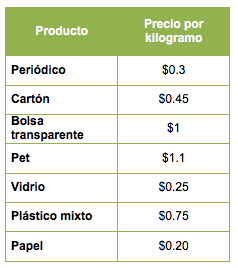
\includegraphics[width=0.3\textwidth]{Images/SINMAT1_U3_AC68_IMG1}
%     \caption{Tabla de precios de los direrentes reciclables.}
%     \label{fig:SINMAT1_U3_AC68_IMG1}
% \end{figure}

\begin{table}[H]
    \centering
    \begin{tabular}{l|c}
        Producto           & Precio por kilogramo \\
        \hline
        Periódico          & \$0.3                \\
        \hline
        Cartón             & \$0.45               \\
        \hline
        Bolsa transparente & \$1                  \\
        \hline
        Pet                & \$1.1                \\
        \hline
        Vidrio             & \$0.25               \\
        \hline
        Plástico mixto     & \$0.75               \\
        \hline
        Papel              & \$0.20               \\
    \end{tabular}
    \caption{Lista con los datos de precio y peso para los productos de reciclaje.}
    \label{table:SINMAT1_U3_AC68_IMG1}
\end{table}
\begin{parts}
    \part  \include*{../parts/question068a01}
    \part  \include*{../parts/question068a02}
    \part  \include*{../parts/question068a03}
    \part  \include*{../parts/question068a04}
    \part  \include*{../parts/question068a05}
    \part  \include*{../parts/question068a06}
    \part  \include*{../parts/question068a07}
\end{parts}